
\section{Introduction}

Vision transformers~\cite{dosovitskiy2020image} (ViT) emerge as an alternative to convolutional neural networks (convnets) in computer vision. 
%
They differ from traditional convnets in many ways, one of which being the patch based processing. Another difference is the aggregation of the image information based on a so-called ``class token''. 
This element correlates with the patches most related to the classification decision. Therefore, the softmax in the self-attention blocks, especially in the last layers, can be used to produce attention maps showing the interaction between the class token and all the patches. 
%
Such maps have been employed for visualization purposes~\cite{caron2021emerging,dosovitskiy2020image}. It gives some hints on which regions of a given image  are employed by a model to make its decision. 
% 
However the interpretability remains loose: producing these maps involves some fusion of multiple softmax in different different layers and heads. 

%
% 
%

\begin{figure}[t]
            \vspace{-0.2ex}
          ~~Original ~~~~~~ ViT-S ~~ ``ResNet-50'' ~~~~~ S60 ~~~~~~~~~~ S60$^\dagger$  \\
         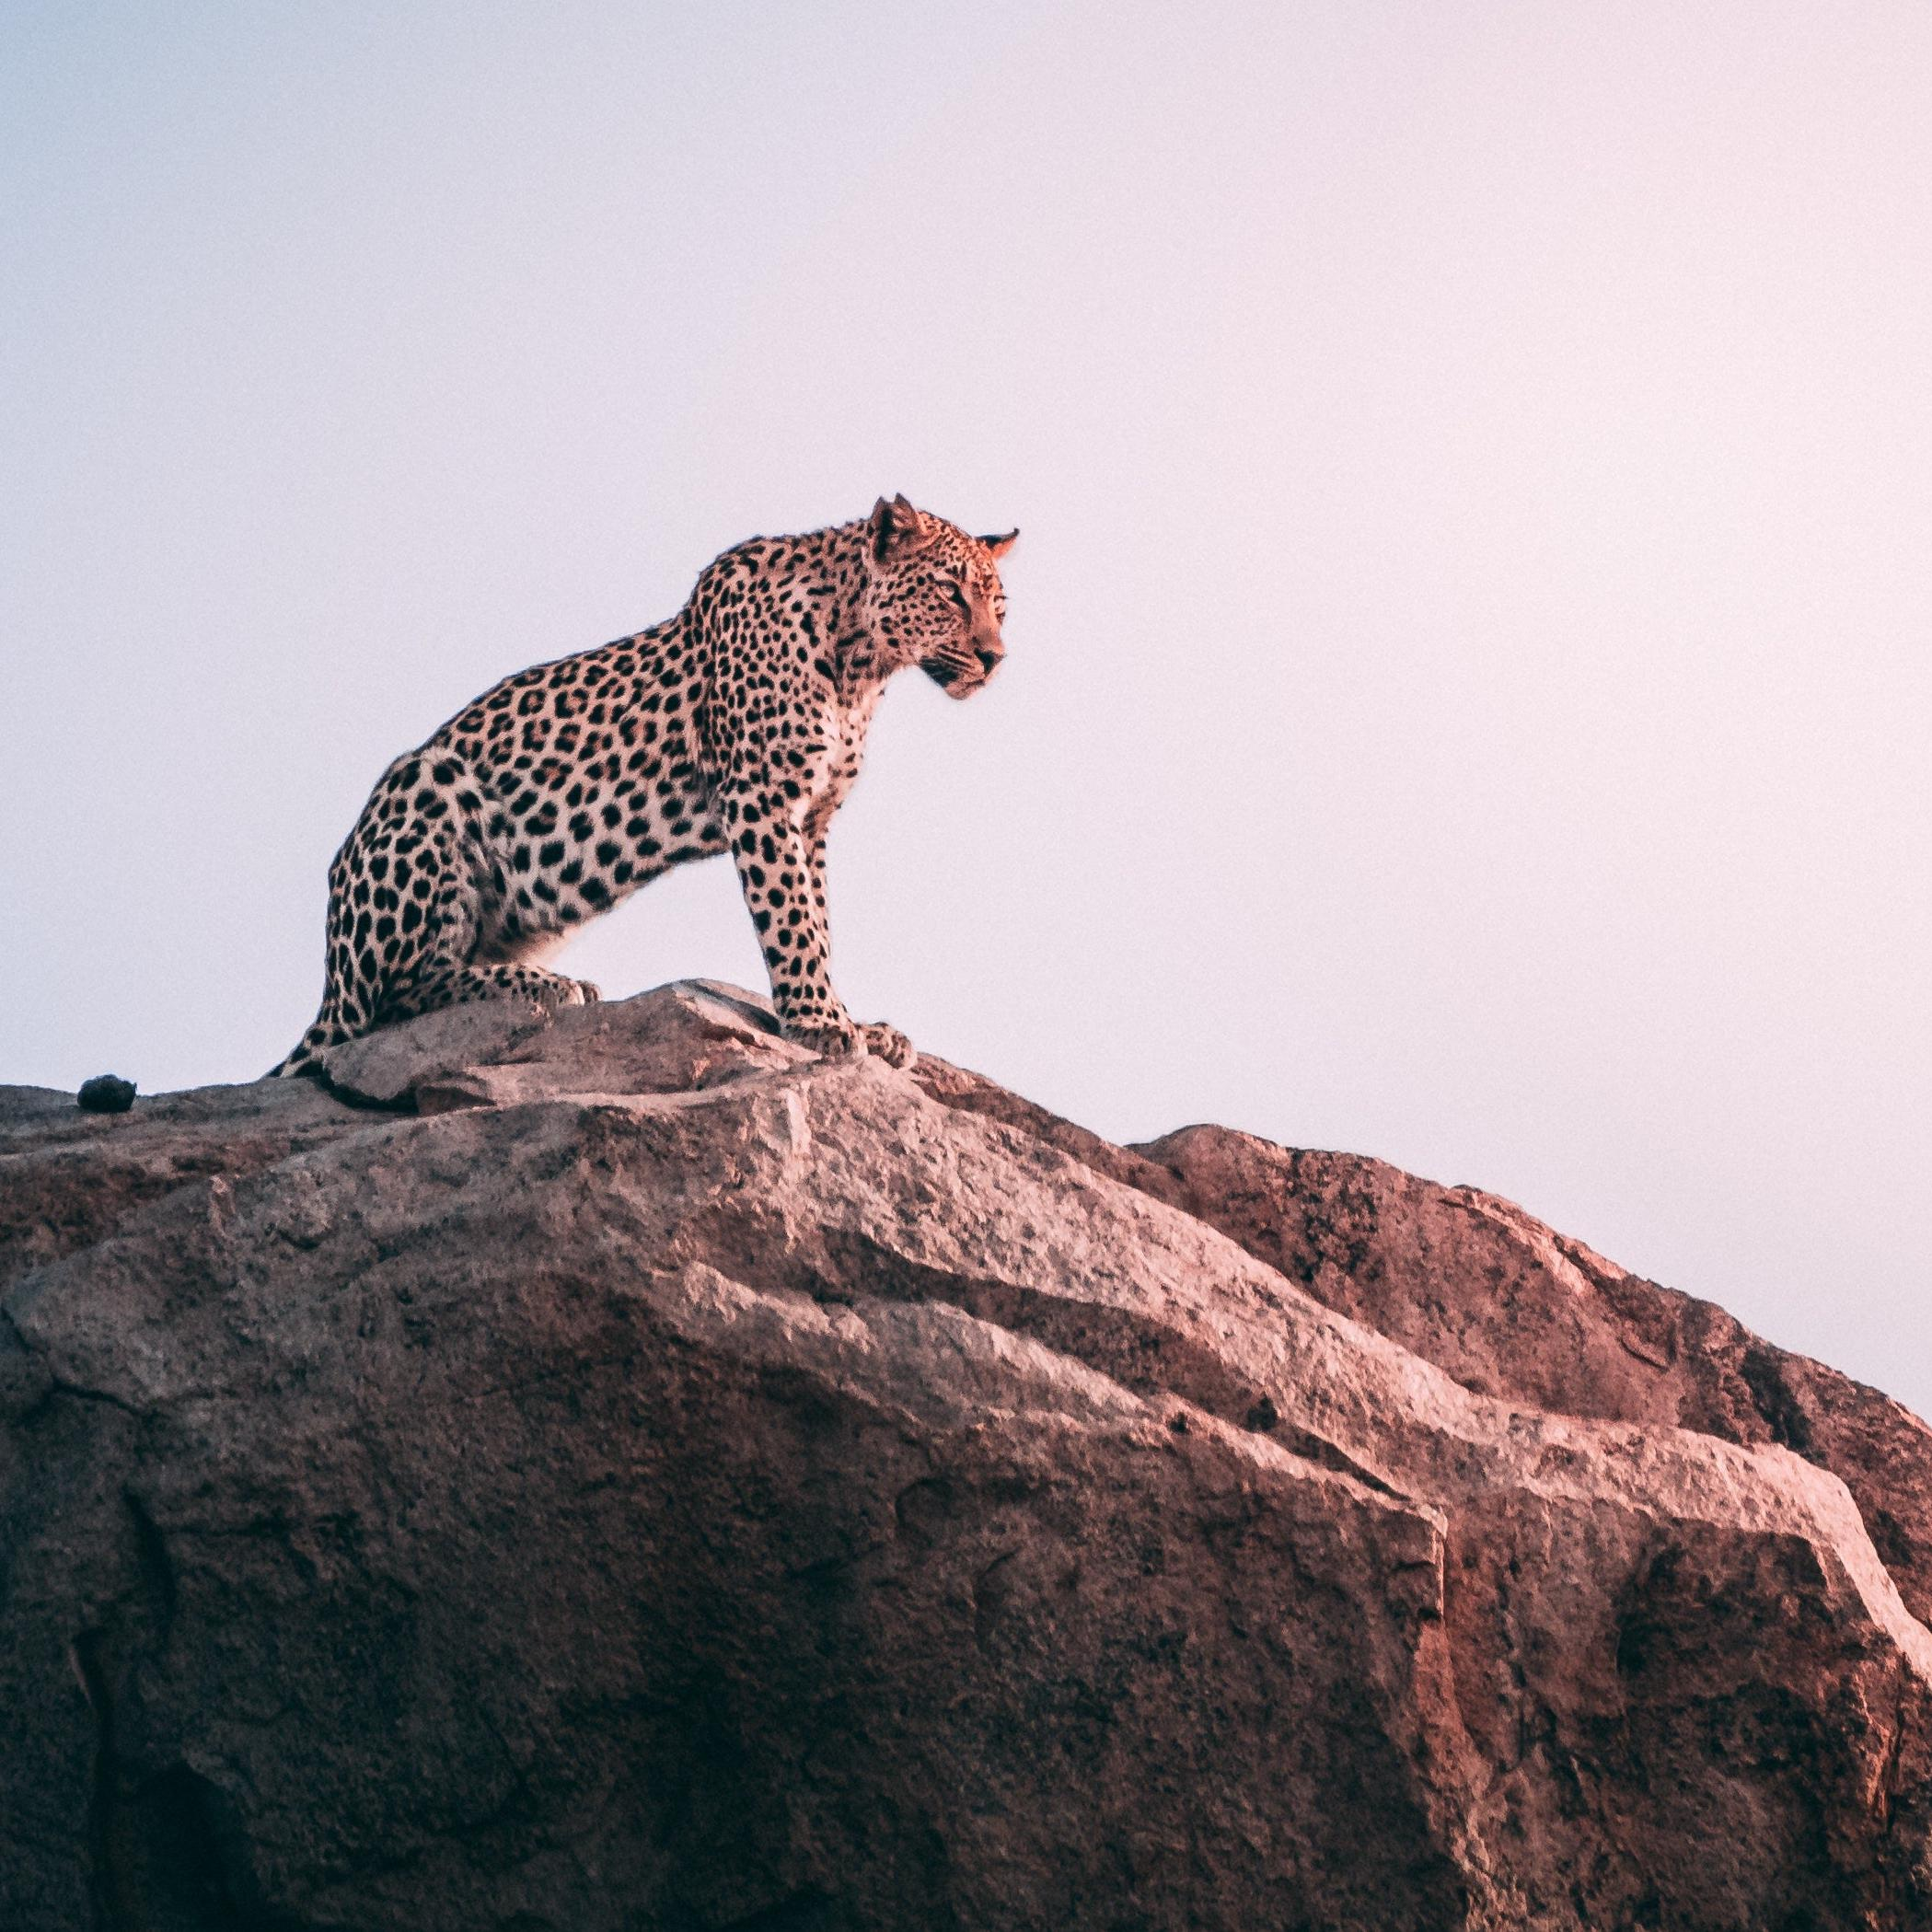
\includegraphics[width = 0.19\linewidth]{figs/attention_fig_main/pexels-geran-de-klerk-2553358.jpg} \hfill
         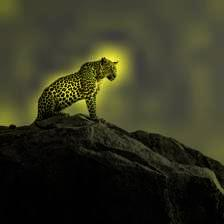
\includegraphics[width = 0.19\linewidth]{figs/attention_fig_main/gray_vit_S_attention_mean_pexels-geran-de-klerk-2553358.jpg} \hfill
          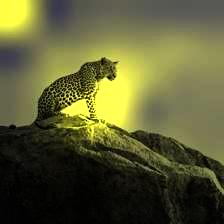
\includegraphics[width = 0.19\linewidth]{figs/attention_fig_main/gray_resnet50_attention_mean_pexels-geran-de-klerk-2553358.jpg} \hfill
         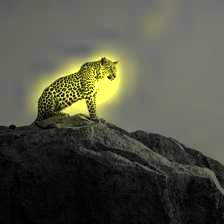
\includegraphics[width = 0.19\linewidth]{figs/attention_fig_main/gray_S60_attention_mean_pexels-geran-de-klerk-2553358.jpg} \hfill
         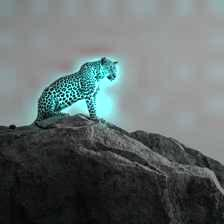
\includegraphics[width = 0.19\linewidth]{figs/attention_fig_main/gray_attn_multi_pexels-geran-de-klerk-2553358.jpg}\\%[0.01cm]
         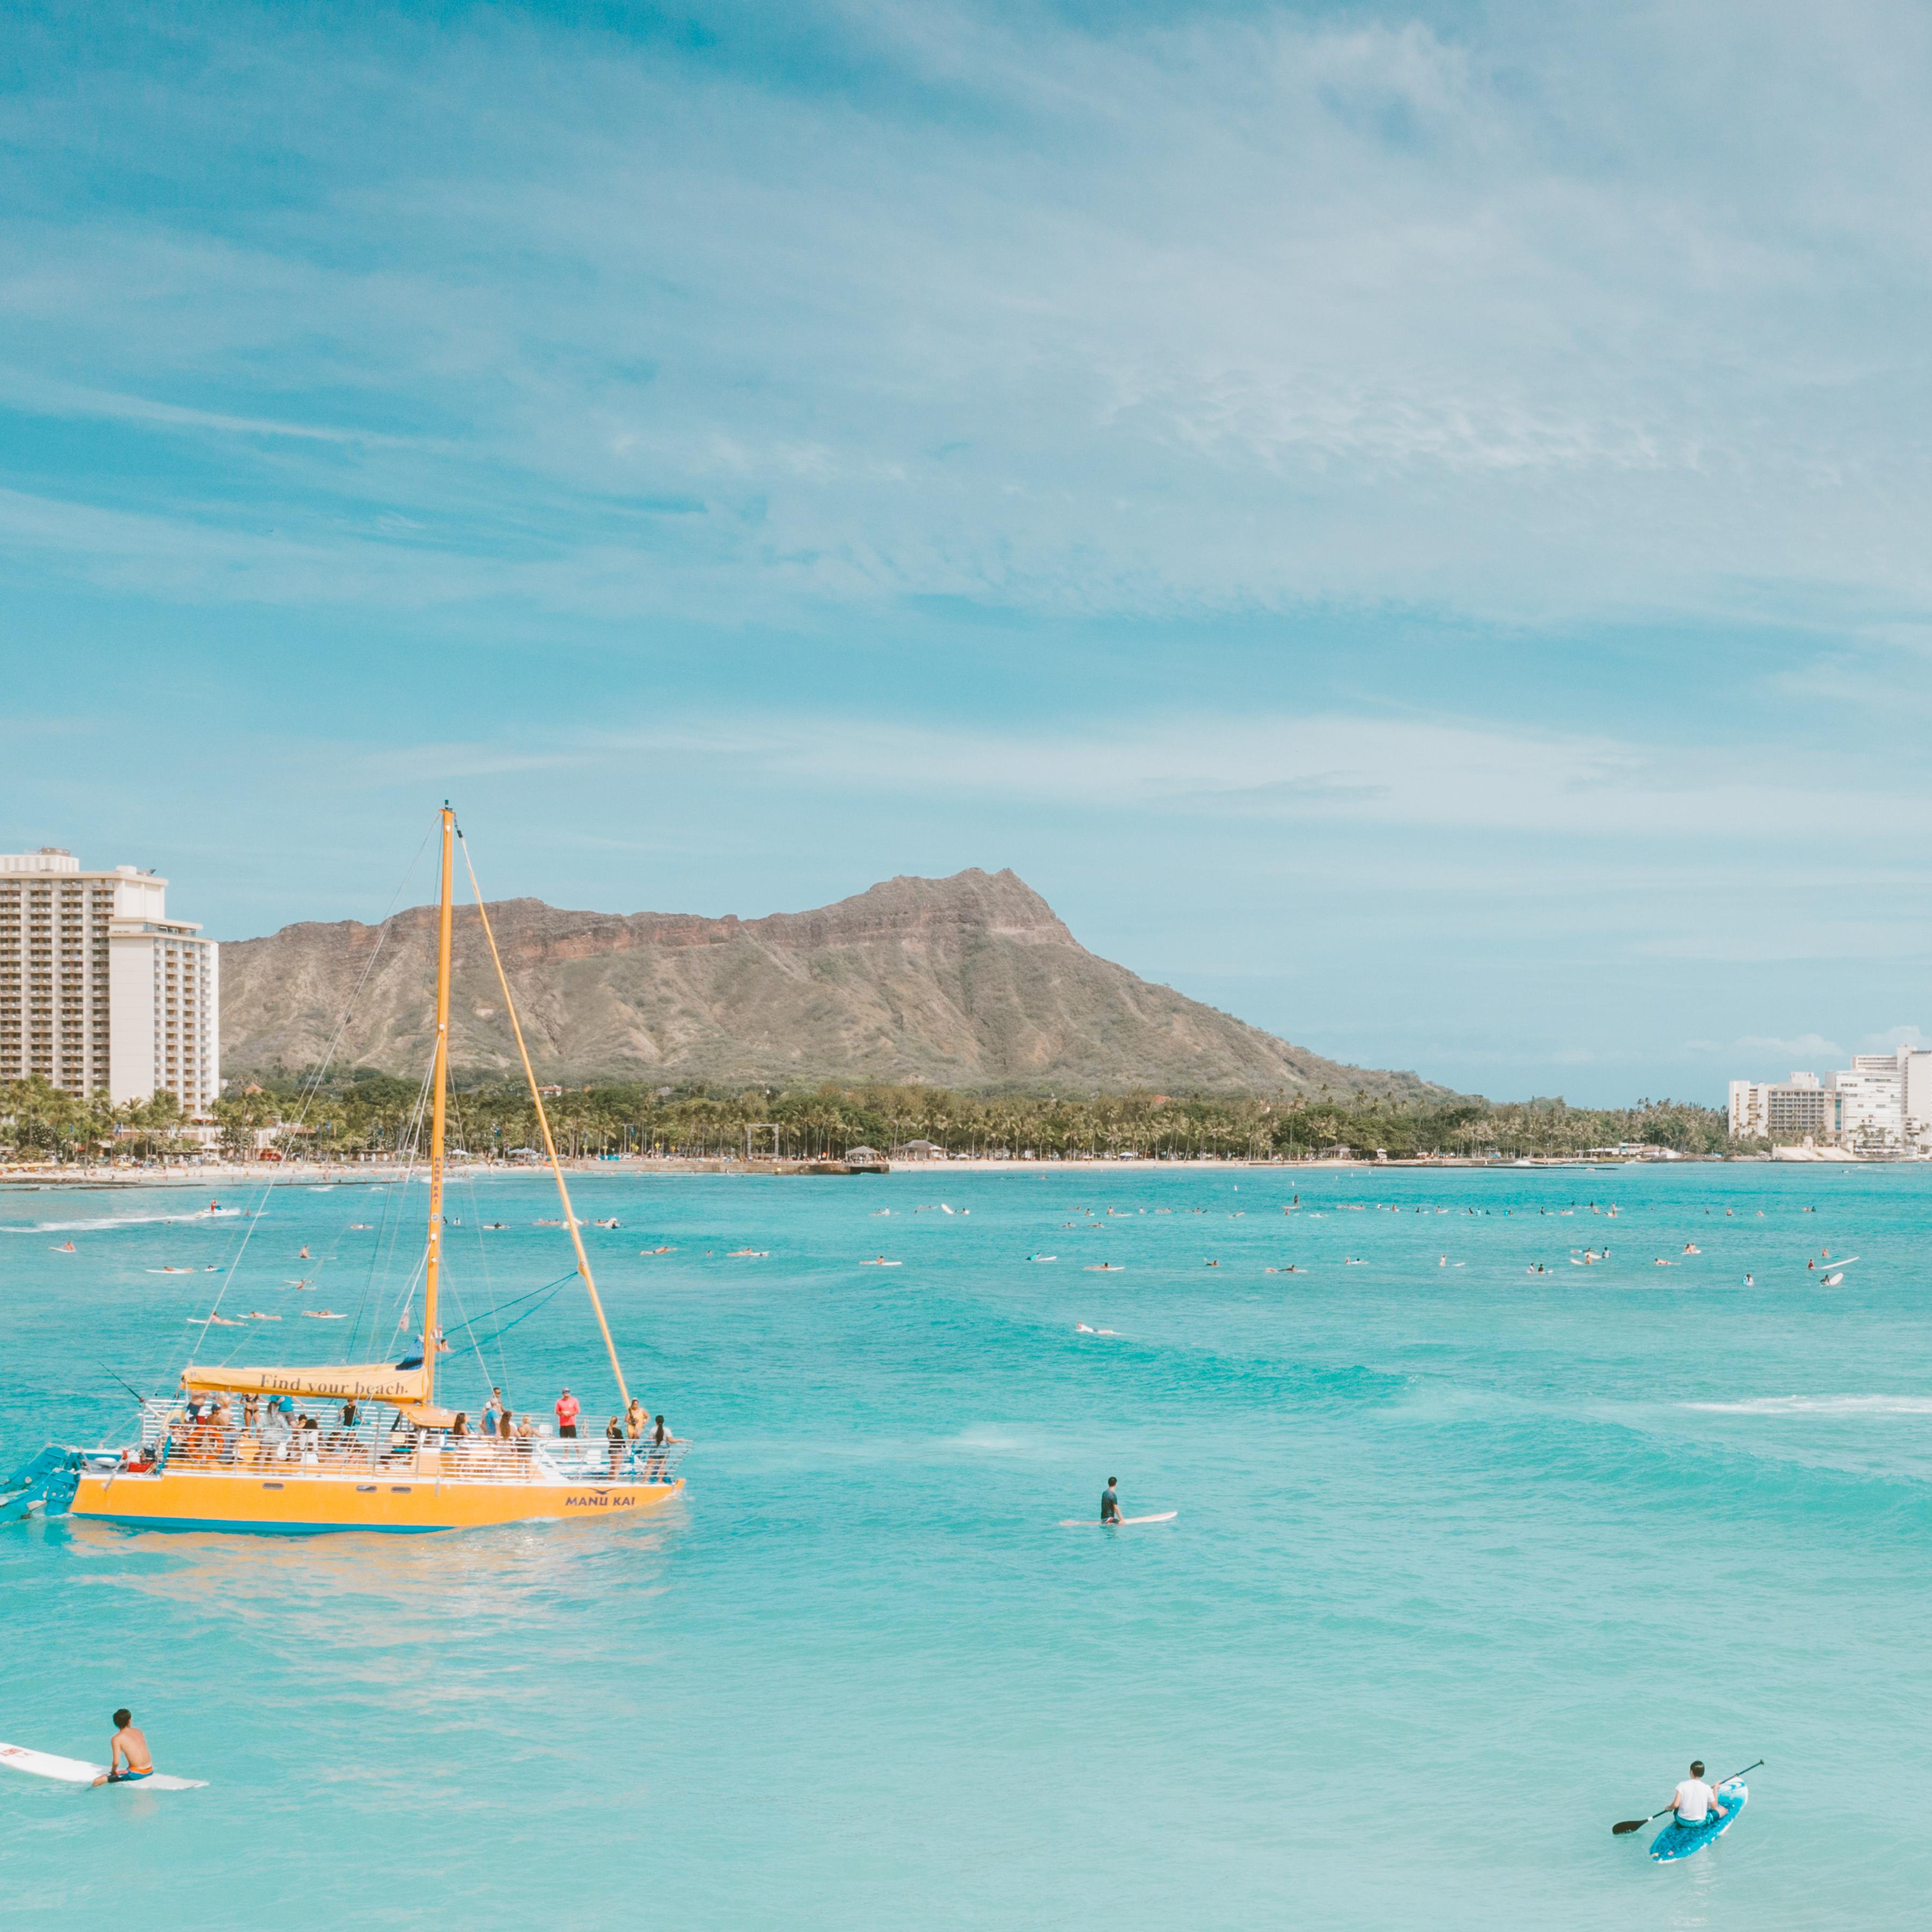
\includegraphics[width = 0.19\linewidth]{figs/attention_fig_main/pexels-jess-vide-4319846.jpg} \hfill
         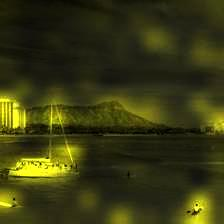
\includegraphics[width = 0.19\linewidth]{figs/attention_fig_main/gray_vit_S_attention_mean_pexels-jess-vide-4319846.jpg} \hfill
        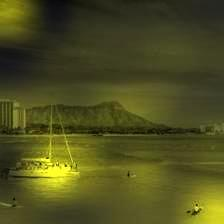
\includegraphics[width = 0.19\linewidth]{figs/attention_fig_main/gray_resnet50_attention_mean_pexels-jess-vide-4319846.jpg} \hfill
         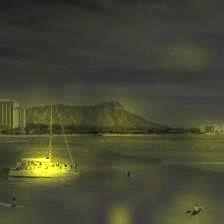
\includegraphics[width = 0.19\linewidth]{figs/attention_fig_main/gray_S60_attention_mean_pexels-jess-vide-4319846.jpg} \hfill
         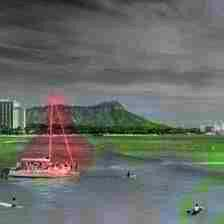
\includegraphics[width = 0.19\linewidth]{figs/attention_fig_main/gray_attn_multi_pexels-jess-vide-4319846.jpg}\\%[0.01cm]
        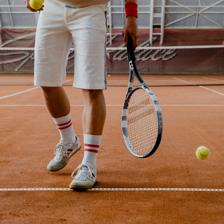
\includegraphics[width = 0.19\linewidth]{figs/attention_fig_main/pexels-cottonbro-5739196.jpg} \hfill
         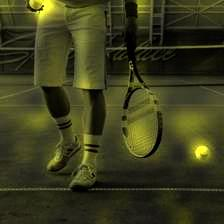
\includegraphics[width = 0.19\linewidth]{figs/attention_fig_main/gray_vit_S_attention_mean_pexels-cottonbro-5739196.jpg} \hfill
        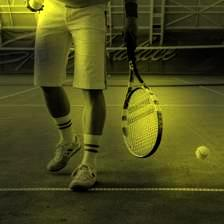
\includegraphics[width = 0.19\linewidth]{figs/attention_fig_main/gray_resnet50_attention_mean_pexels-cottonbro-5739196.jpg} \hfill
         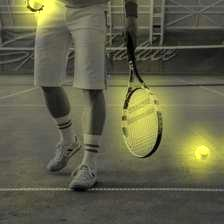
\includegraphics[width = 0.19\linewidth]{figs/attention_fig_main/gray_S60_attention_mean_pexels-cottonbro-5739196.jpg} \hfill
         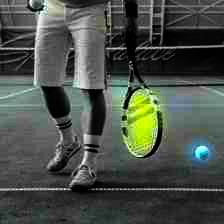
\includegraphics[width = 0.19\linewidth]{figs/attention_fig_main/gray_attn_multi_pexels-cottonbro-5739196.jpg}\\%[0.01cm]      
        
\includegraphics[width = 0.19\linewidth]{figs/attention_fig_main/pexels-pixabay-257894.jpg} \hfill
         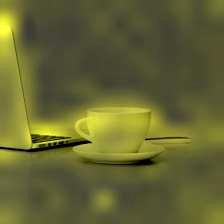
\includegraphics[width = 0.19\linewidth]{figs/attention_fig_main/gray_vit_S_attention_mean_pexels-pixabay-257894.jpg} \hfill
        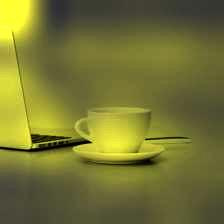
\includegraphics[width = 0.19\linewidth]{figs/attention_fig_main/gray_resnet50_attention_mean_pexels-pixabay-257894.jpg} \hfill
         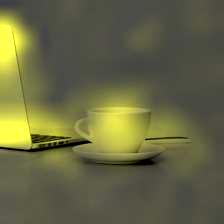
\includegraphics[width = 0.19\linewidth]{figs/attention_fig_main/gray_S60_attention_mean_pexels-pixabay-257894.jpg} \hfill
         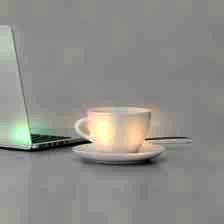
\includegraphics[width = 0.19\linewidth]{figs/attention_fig_main/gray_attn_multi_pexels-pixabay-257894.jpg}\\%[0.01cm]                
    \vspace{-3.0ex}
    \caption{We augment convolutional neural networks with a learned attention-based aggregation layer. We visualize the attention maps for classification for diverse models. We first extract attention maps from a regular ViT-S~\cite{dosovitskiy2020image,Touvron2020TrainingDI} with Dino-style~\cite{caron2021emerging} vizualizations. Then we consider convnets in which we replace the average pooling by our learned attention-based aggregation layer. Unlike ViT, this layer directly provides the contribution of the patches in the weighted pooling. 
    This is shown for a ``ResNet-50~\cite{He2016ResNet}'', and with our new simple patch-based model (\ournet{}-S60) that we introduce to increase the attention map resolution. 
    We can specialize this attention per class, as shown with S60$\dagger$. 
    \label{fig:attention_maps_intro}}
\end{figure}



In this paper, we want to provide similar vizualization properties to convnets: %
we augment convnets with an attention map.  %
More precisely we replace the usual average pooling layer by an attention-based layer. 
Indeed, nothing in the convnets design precludes replacing their pooling by attention~\cite{Bello2019AttentionAC}. 
We simplify the design of this attention-based pooling layer such that it explicitly provides the weights of the different patches. %
Compared to ViT, for which the aggregation is performed across multiple layers and heads, our proposal offers a single weight per patch, and therefore a simple way to interpret the attention map: it is the respective contribution of each patch in the weighted sum summarizing the images. 
%
This treatment allows the model to deal with visual objects separately or jointly: if we use one token for each class instead of a single token, as exemplified in Figures~\ref{fig:attention_maps_intro} and~\ref{fig:visu_attention}, then we obtain an attention weight per patch for each possible class. In our main proposal we mostly focus on the single token case, which is more directly related to the classification decision. 


In Figure~\ref{fig:attention_maps_intro}, we show the attention maps extracted from ViT by using a visualization procedure inspired by Caron et al.~\cite{caron2021emerging}. It involves some post-processing as there are multiple layers and heads providing patch weights. 
Then we show a "ResNet-50" augmented by adding our attention-based aggregation layer. Its hierarchical design leads to a low-resolution  attention map with artefacts: We need an architecture producing a higher-resolution feature maps in order to better leverage the proposed attention-based pooling. 
 
% 
For this purpose we introduce a simple patch-based convolutional architecture\footnote{Existing patch-based architectures such as MLP designs~\cite{tolstikhin2021MLPMixer,Touvron2021ResMLPFN,ding2021repmlp} or  convMixer~\cite{anonymous2022patches} yield poor accuracy/complexity trade-offs. } that keeps the input resolution constant throughout the network.
This design departs from the historical pyramidal architectures of LeNet~\cite{lecun1989backpropagation}, AlexNet~\cite{Krizhevsky2012AlexNet} or ResNet~\cite{He2016ResNet,He2016IdentityMappings}, to name only a few. 
Their pyramidal design was motivated by the importance of reducing the resolution while increasing the working dimensionality.
That allowed one to maintain a moderate complexity while progressively increasing the working dimensionality, making the space large enough to be separable by a linear classifier.
In our case, we simplify the trunk after a small pre-processing stage that produces the patches. We adopt the same dimensionality throughout all the trunk, fixing it equal to that of the final layer, e.g. our aggregation layer.
We refer to it as \ournet, see Figure~\ref{fig:full_model} for an overview of this network. 
%

In summary, we make the following contributions: 
\begin{itemize}
    \item We revisit the final pooling layer in convnets by presenting a learned, attention-based pooling;
    
    \item We propose a slight adaptation of our attention-based pooling in order to have one attention map per class, offering a better interpretability of the predictions;
    
    \item We propose an architecture, \ournet{}, with a simple patch-based design (two parameters: depth and width) and a simple training recipe: same learning rate for all our
models, a single regularization parameter. 
\end{itemize}

\noindent We share the architecture definition and pretrained models\footnote{\url{https://github.com/facebookresearch/deit}}. 

\begin{figure}[t]

         \vspace{-0.2ex}
             ~~~~Original~~~~~~~~~~~~~Top-1~~~~~~~~~~~~~~Top-2~~~~~~~~~~~~~~Top-3\\
              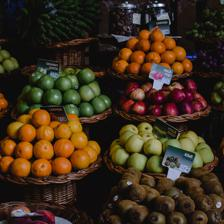
\includegraphics[width=0.24\linewidth]{figs/multiclass/pexels-eva-elijas-6148830.jpg} \hfill%
              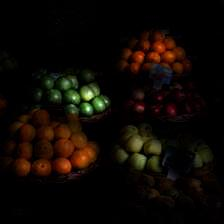
\includegraphics[width=0.24\linewidth]{figs/multiclass/attn0_multi_pexels-eva-elijas-6148830.jpg} \hfill %&
              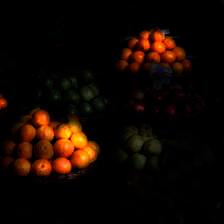
\includegraphics[width=0.24\linewidth]{figs/multiclass/attn1_multi_pexels-eva-elijas-6148830.jpg} \hfill %&
              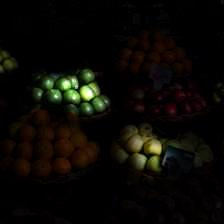
\includegraphics[width=0.24\linewidth]{figs/multiclass/attn2_multi_pexels-eva-elijas-6148830.jpg} \\[-5pt] % 
               {\scriptsize \phantom{0} \hspace{0.215\linewidth} grocery\,store\,(46.7\%) ~~~ orange\,(6.0\%) ~~~~ Granny\,Smith\,(4.9\%)} \\ %
              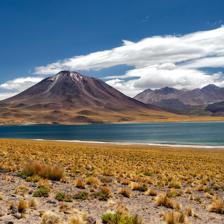
\includegraphics[width=0.24\linewidth]{figs/multiclass/pexels-andre-ulysses-de-salis-7865866.jpg} \hfill%
              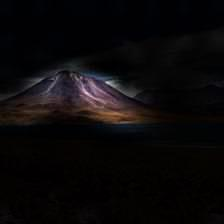
\includegraphics[width=0.24\linewidth]{figs/multiclass/attn0_multi_pexels-andre-ulysses-de-salis-7865866.jpg} \hfill %
              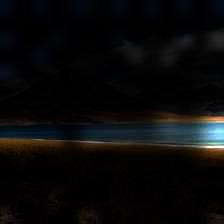
\includegraphics[width=0.24\linewidth]{figs/multiclass/attn1_multi_pexels-andre-ulysses-de-salis-7865866.jpg} \hfill %
              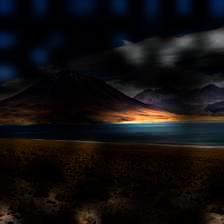
\includegraphics[width=0.24\linewidth]{figs/multiclass/attn2_multi_pexels-andre-ulysses-de-salis-7865866.jpg}  \\[-5pt] % 
             {\scriptsize \phantom{0} \hspace{0.215\linewidth} ~~~volcano\,(86.6\%) ~~~~~~~~~ lakeside\,(0.4\%) ~~~~~~~~ valley\,(0.2\%)}%
              \\
              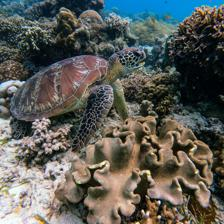
\includegraphics[width=0.24\linewidth]{figs/multiclass/pexels-keemkai-villadums-2435728.jpg} \hfill%
              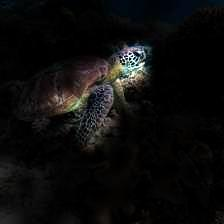
\includegraphics[width=0.24\linewidth]{figs/multiclass/attn0_multi_pexels-keemkai-villadums-2435728.jpg} \hfill %
              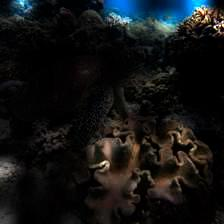
\includegraphics[width=0.24\linewidth]{figs/multiclass/attn1_multi_pexels-keemkai-villadums-2435728.jpg} \hfill %
              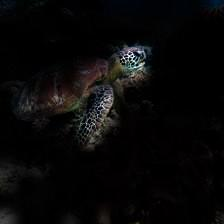
\includegraphics[width=0.24\linewidth]{figs/multiclass/attn2_multi_pexels-keemkai-villadums-2435728.jpg}  \\[-5pt] % 
             {\scriptsize \phantom{0} \hspace{0.18\linewidth} loggerhead\,turtle\,(66.4\%) ~~coral\,reef\,(15.2\%) ~~leathery\,turtle\,(1.3\%)}%
              \\
 % 
         %
          
        \vspace{-3ex}
    \caption{
    We provide three images for which the attention-based aggregation stage is specialized so as to provide one attention map per class.  We display the attention for the top-3 classes w.r.t. the model prediction. 
    \label{fig:visu_attention}}
 % 
\end{figure}
